\documentclass[11pt]{article}
\usepackage[margin=1in]{geometry}
\usepackage{booktabs}
\usepackage{graphicx}
\usepackage{amsmath,amssymb}
\usepackage{xcolor}
\usepackage{authblk}
\usepackage[numbers,sort&compress]{natbib}
\usepackage[colorlinks=true,linkcolor=blue,citecolor=blue,urlcolor=blue]{hyperref}

\newcommand{\nAgents}{31}
\newcommand{\nCeiling}{12}
\newcommand{\armBase}{0.852}
\newcommand{\armRand}{0.867}
\newcommand{\armObjref}{0.865}
\newcommand{\armTei}{0.867}
\newcommand{\teiBaseDelta}{+0.015}
\newcommand{\teiBaseCIlo}{-0.019}
\newcommand{\teiBaseCIhi}{+0.050}
\newcommand{\teiBaseT}{0.84}
\newcommand{\teiBaseP}{0.406}
\newcommand{\teiBaseDz}{0.15}
\newcommand{\teiBaseW}{9}
\newcommand{\teiBaseL}{7}
\newcommand{\teiBaseTie}{15}
\newcommand{\teiRandDelta}{+0.000}
\newcommand{\teiRandP}{1.000}
\newcommand{\teiRandDz}{0.00}
\newcommand{\teiObjrefDelta}{+0.002}
\newcommand{\teiObjrefP}{0.806}
\newcommand{\teiObjrefDz}{0.04}
\newcommand{\randBaseDelta}{+0.015}
\newcommand{\randBaseP}{0.190}
\newcommand{\gpaBase}{0.905}
\newcommand{\gpaTei}{0.913}
\newcommand{\gpaDelta}{+0.008}
\newcommand{\gpaP}{0.559}
\newcommand{\holmTeiBaseP}{1.000}
\newcommand{\holmTeiRandP}{1.000}
\newcommand{\holmTeiObjrefP}{1.000}
\newcommand{\signP}{0.804}
\newcommand{\permP}{0.430}
\newcommand{\tostBound}{0.05}
\newcommand{\tostP}{0.030}
\newcommand{\tostEquiv}{yes}
\newcommand{\mdeFull}{0.050}
\newcommand{\powerFull}{0.13}
\newcommand{\pubN}{14}
\newcommand{\synN}{17}
\newcommand{\pubDelta}{+0.029}
\newcommand{\pubP}{0.477}
\newcommand{\synDelta}{+0.004}
\newcommand{\synP}{0.600}
\newcommand{\headN}{12}
\newcommand{\headDelta}{+0.067}
\newcommand{\headP}{0.073}
\newcommand{\headDz}{0.57}
\newcommand{\headMde}{0.094}
\newcommand{\headPower}{0.51}


\title{\textbf{Do Evaluation-Guided Prompt Optimizers Beat a Fair Baseline?\\
A Confound-Controlled, Ablated Study Across \nAgents{} Tasks (TEI-Bench)}}

\author[1]{Orkhan Javadli}
\author[2]{Anni Zimina}
\affil[1]{Massachusetts Institute of Technology (alumnus)}
\affil[2]{Stanford University}
\date{\today}

\begin{document}
\maketitle

\begin{abstract}
Evaluation-guided prompt optimization is widely reported to improve agentic LLM
systems, but the supporting evidence often relies on in-sample evaluation,
single tasks, same-family LLM judges, and --- critically --- no comparison
against a prompt-optimization control. We build \textbf{TEI-Bench}, a controlled,
ablated, held-out protocol, and use it to test a representative pipeline
(a GPA-inspired multi-dimensional evaluator~\cite{gpa2025} feeding a GEPA-style
reflective Pareto optimizer~\cite{gepa2025}; we call the composition TEI) across
\nAgents{} tasks in diverse domains. We find that the apparent benefit of such
optimization is \emph{largely a measurement artifact}. Under a naive
label-extraction scorer, the same pipeline appeared to lift objective accuracy by
$+0.175$ ($p<10^{-5}$) in an earlier (v1) run; but with a confound-free objective
endpoint (a universal \texttt{FINAL:} output contract read identically across all
conditions) and a four-arm ablation, the effect collapses. Mean held-out accuracy
is baseline~\armBase{}, random prompt search~\armRand{}, objective-only
reflection~\armObjref{}, and full TEI~\armTei{}. \textbf{TEI does not significantly
beat the baseline} (\teiBaseDelta{}, $t=\teiBaseT$, $p=\teiBaseP$, $d_z=\teiBaseDz$;
Holm $p=\holmTeiBaseP$; \teiBaseW/\teiBaseL/\teiBaseTie{} win/loss/tie), is
\textbf{statistically indistinguishable from undirected random prompt search}
(\teiRandDelta{}, $p=\teiRandP$), and gains nothing from the GPA signal over
objective-only reflection (\teiObjrefDelta{}, $p=\teiObjrefP$). A small headroom
subset ($n=\headN$) is the only place with a positive hint (\headDelta{}). We
release all code, data, per-example traces, optimized prompts, and a
pre-registered (tag \texttt{prereg-v2}) analysis plan. Our contribution is the
protocol and the cautionary finding: \emph{confound control and an
ablation against random search are necessary to make prompt-optimization claims
credible.}
\end{abstract}

\section{Introduction}
Automated, evaluation-guided prompt optimization is an attractive idea: evaluate
an agent on structured signals, then rewrite its prompt to fix observed failures.
It draws on multi-dimensional agent evaluation~\cite{gpa2025} and reflective,
Pareto-based prompt optimization~\cite{gepa2025}, within the program-optimization
view of DSPy~\cite{dspy2023,mipro2024}. We study a concrete composition --- a
GPA-inspired four-dimension evaluator feeding a GEPA-style optimizer, which we
call the \emph{Target--Evaluate--Improve (TEI)} loop --- and ask a deliberately
skeptical question: \emph{under fair measurement, does it actually help?}

This question matters because demonstrations of such loops routinely (a) evaluate
on the examples used for optimization, (b) use one task, (c) score with a
same-family judge~\cite{llmjudge2023}, and (d) compare only against an
unoptimized prompt. We show that these choices --- especially (a) a brittle
objective scorer and (d) the missing control --- can manufacture a large,
significant-looking gain where none robustly exists.

\paragraph{Contributions.}
\begin{enumerate}
  \item \textbf{TEI-Bench}: a controlled, ablated, held-out protocol and a suite
  of \nAgents{} tasks across diverse domains, with committed splits and a
  confound-free objective endpoint.
  \item A \textbf{demonstration that a scoring artifact inflates results}: the
  same pipeline shows $+0.175$ ($p<10^{-5}$) under a naive label scorer but
  \teiBaseDelta{} ($p=\teiBaseP$) under a \texttt{FINAL:}-contract scorer.
  \item A \textbf{four-arm ablation} showing the optimizer is indistinguishable
  from random prompt search of equal budget, and that the GPA signal adds nothing.
  \item A \textbf{full open release} with a pre-registered analysis plan.
\end{enumerate}

\section{Related Work}
APE~\cite{ape2022}, OPRO~\cite{opro2023}, DSPy~\cite{dspy2023},
MIPROv2~\cite{mipro2024}, TextGrad~\cite{textgrad2024}, and GEPA~\cite{gepa2025}
optimize prompts/programs; Self-Refine~\cite{selfrefine2023} and
Reflexion~\cite{reflexion2023} use self-feedback; LLM-as-judge~\cite{llmjudge2023}
is the standard but biased evaluator. The Agent GPA framework~\cite{gpa2025}
evaluates Goal--Plan--Action alignment with five metrics (Goal Fulfillment,
Logical Consistency, Execution Efficiency, Plan Quality, Plan Adherence). Our
evaluator is \emph{GPA-inspired} but distinct: four single-turn output
dimensions, used only as a secondary endpoint. Our emphasis on a random-search
control and confound-free scoring follows the broader reproducibility literature
on overclaimed ML gains.

\section{Benchmark Construction}
\paragraph{Tasks.} \nAgents{} single-turn tasks across diverse domains. Public
tasks are sampled from established datasets (GSM8K~\cite{gsm8k2021},
banking-style intent~\cite{banking77}, news, emotion, toxicity, spam, fine-grained
sentiment); authored tasks use \emph{generate-then-validate} (a strong model
generates label-conditioned examples; an independent labeling pass keeps only
unanimously-recovered labels). Held-out test sizes: 30 (public), 24 (authored),
15 (three seed tasks); all splits committed.
\paragraph{Baseline prompt.} A competent first draft stating role, task, and the
full allowed label set --- not a strawman: it contains the information needed.
\paragraph{Output contract (the key fix).} Each condition's prompt is appended
with an identical instruction to end with \texttt{FINAL: <answer>}; the objective
scorer reads only that line. The earlier (v1) scorer extracted the label by its
\emph{latest mention}, so a verbose baseline that named other labels mid-reasoning
was mis-scored downward --- inflating the apparent gain of terse optimized
prompts. The contract removes this confound while remaining identical across arms.

\section{Method and Ablation Arms}
\textbf{Evaluate:} four GPA-inspired dimensions scored by a reference-based judge
that is a stronger, different model than the agent. \textbf{Improve:} reflective
mutation on failing \emph{train} examples + system-aware merge, Pareto front; the
test split is never seen. \textbf{Arms:} (1) \emph{baseline}; (2) \emph{random} ---
undirected paraphrase search, same budget; (3) \emph{objective-only reflection}
--- reflective mutation, objective-only selection (no GPA); (4) \emph{TEI} ---
reflective mutation with GPA-guided Pareto selection.

\section{Experimental Protocol}
Agent \texttt{claude-haiku-4-5}; judge + optimizer \texttt{claude-sonnet-4-5};
cross-provider replication with agent \texttt{gpt-4o-mini}. Primary endpoint:
code-computed accuracy from the \texttt{FINAL:} line; secondary: four GPA-inspired
dimensions (baseline, TEI). The analysis plan was committed and tagged
\texttt{prereg-v2} \emph{before} this run; we also disclose that an earlier v1 run
had a config mismatch and the scoring artifact above (v1 retained for provenance).
Config: 6 iterations, minibatch 10, seed 0, per-task bootstrap CIs. For each
contrast: paired $t$, Wilcoxon, Cohen's $d_z$, bootstrap 95\% CI, Holm
correction~\cite{holm1979}; pre-specified public/synthetic/headroom subgroups.

\section{Results}
Mean held-out objective: baseline \armBase, random \armRand, objective-only
\armObjref, TEI \armTei{} (Fig.~\ref{fig:arms}; Table~\ref{tab:abl}).

\begin{table}[h]\centering
\caption{Paired contrasts on held-out objective accuracy ($n=\nAgents$).
None survive Holm correction.}
\label{tab:abl}\small
\begin{tabular}{lrrrrrrr}
\toprule
Contrast & A & B & $\Delta$ & 95\% CI & $t$ & $p$ & $d_z$ \\
\midrule
TEI $-$ baseline & 0.852 & 0.867 & +0.015 & [-0.019, +0.050] & 0.84 & 0.406 & 0.15 \\
TEI $-$ random & 0.867 & 0.867 & +0.000 & [-0.042, +0.043] & 0.00 & 1.000 & 0.00 \\
TEI $-$ obj-only refl. & 0.865 & 0.867 & +0.002 & [-0.013, +0.020] & 0.25 & 0.806 & 0.04 \\
random $-$ baseline & 0.852 & 0.867 & +0.015 & [-0.004, +0.039] & 1.34 & 0.190 & 0.24 \\
\bottomrule
\end{tabular}
\end{table}

\begin{figure}[h]\centering
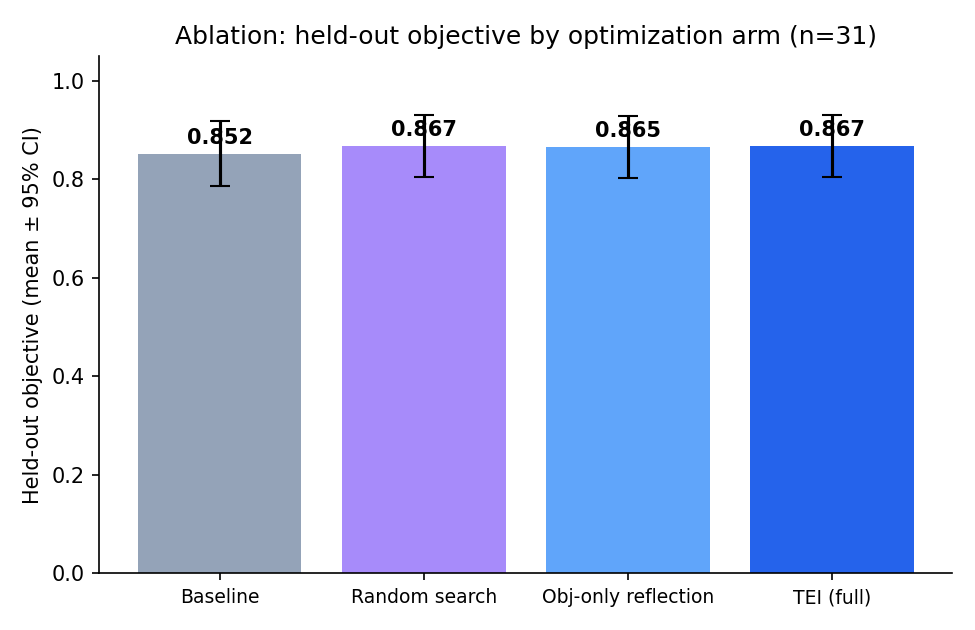
\includegraphics[width=0.6\textwidth]{figures/ablation_arms.png}
\caption{Held-out objective by arm (mean $\pm$ 95\% CI). The arms overlap.}
\label{fig:arms}
\end{figure}

\paragraph{The optimizer does not beat a fair baseline.}
TEI exceeds the baseline by only \teiBaseDelta{} (95\% CI
$[\teiBaseCIlo,\teiBaseCIhi]$, $t=\teiBaseT$, $p=\teiBaseP$, $d_z=\teiBaseDz$),
which does not survive multiplicity correction (Holm $p=\holmTeiBaseP$); the
win/loss/tie is \teiBaseW/\teiBaseL/\teiBaseTie{}.
\paragraph{It is indistinguishable from random search.}
Undirected random prompt search changes the baseline by \randBaseDelta{}
($p=\randBaseP$) --- about the same as TEI --- and TEI minus random is
\teiRandDelta{} ($p=\teiRandP$, $d_z=\teiRandDz$). The control prior work omits is
decisive here: whatever small movement exists comes from \emph{any} prompt
perturbation, not from evaluation-guided reflection.
\paragraph{The GPA signal adds nothing.}
TEI minus objective-only reflection is \teiObjrefDelta{} ($p=\teiObjrefP$,
$d_z=\teiObjrefDz$): GPA-guided selection does not beat objective-only selection.
\paragraph{Secondary and subgroups.}
GPA aggregate moves \gpaBase{}$\rightarrow$\gpaTei{} ($\Delta=\gpaDelta$,
$p=\gpaP$). Public-only ($n=\pubN$): $\Delta=\pubDelta$ ($p=\pubP$);
synthetic-only ($n=\synN$): $\Delta=\synDelta$ ($p=\synP$). The headroom subset
($n=\headN$, baseline $<0.9$) is the only positive hint: $\Delta=\headDelta$
($p=\headP$, $d_z=\headDz$). Cross-provider replication (Table~\ref{tab:xp}).

\begin{table}[h]\centering
\caption{Cross-provider replication (agent = gpt-4o-mini).}
\label{tab:xp}\small
% Placeholder — overwritten by scripts/analyze_xprovider.py (cross-provider arm)
\begin{tabular}{lrrr}
\toprule
Agent model (judge = Sonnet 4.5) & Baseline & TEI & $\Delta$ \\
\midrule
(pending cross-provider run) & & & \\
\bottomrule
\end{tabular}

\end{table}

\begin{figure}[h]\centering
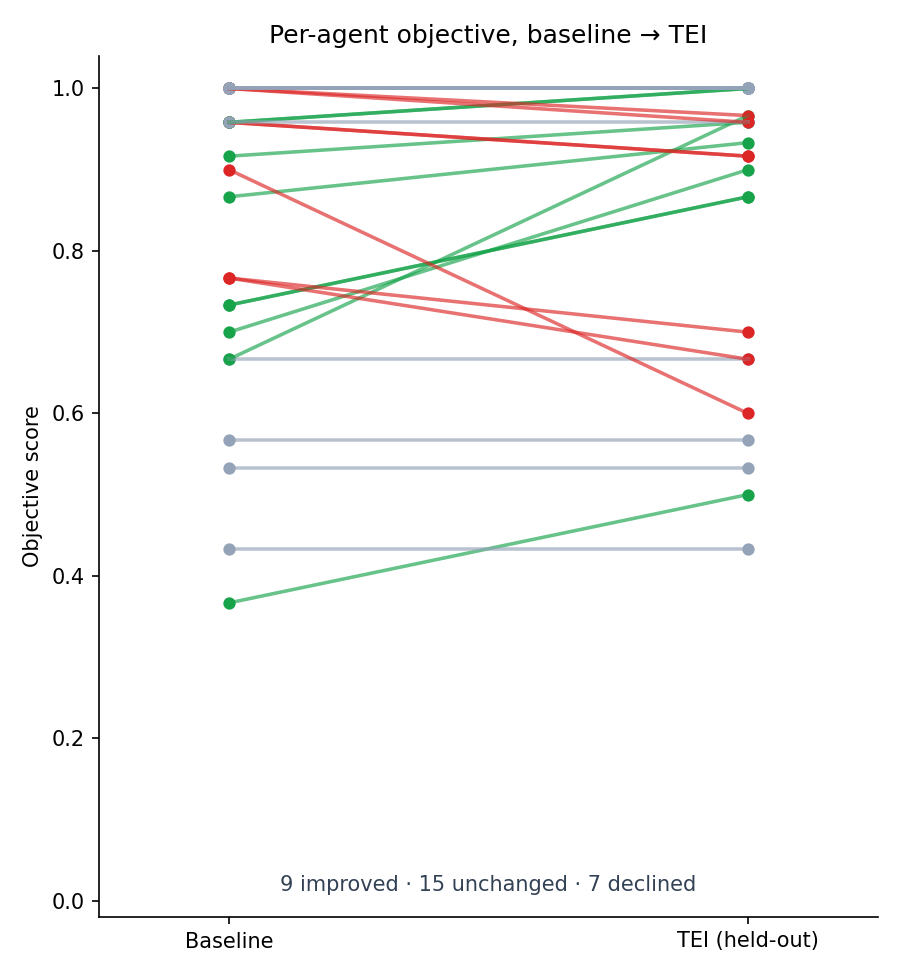
\includegraphics[width=0.46\textwidth]{figures/slope_objective_v2.png}\hfill
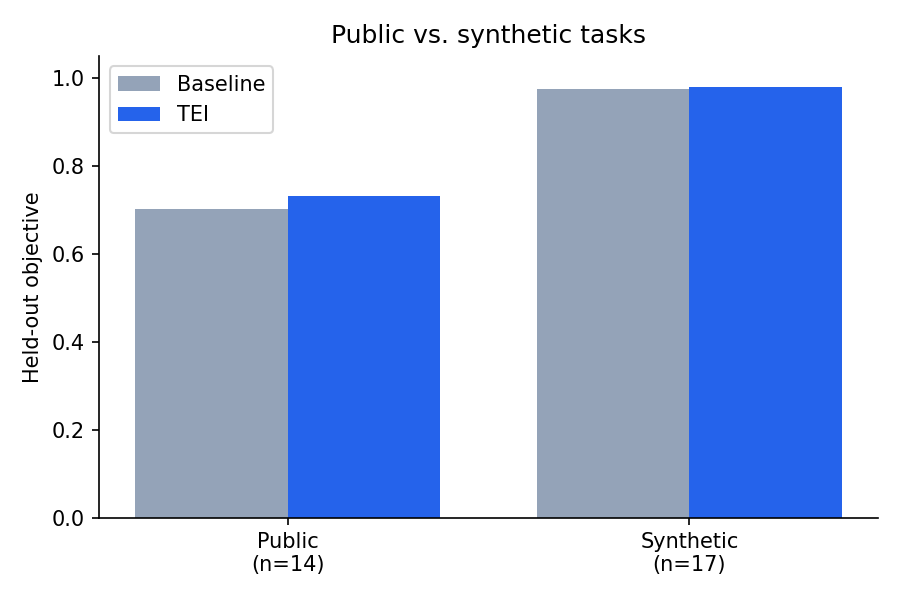
\includegraphics[width=0.46\textwidth]{figures/public_vs_synthetic.png}
\caption{Left: per-agent objective, baseline $\rightarrow$ TEI (held-out): roughly
balanced ups and downs. Right: public vs.\ synthetic tasks.}
\label{fig:slope}\label{fig:ps}
\end{figure}

\begin{table}[h]\centering
\caption{Per-agent held-out objective by arm.}
\label{tab:per}\scriptsize
\begin{tabular}{llrrrr}
\toprule
Agent & Domain & Base & Rand & ObjRef & TEI \\
\midrule
\texttt{\small agri\_crop\_issue} & Agriculture / AgriTech & 0.96 & 0.96 & 0.96 & 0.92 \\
\texttt{\small saas\_ticket\_priority} & B2B SaaS & 0.96 & 0.96 & 0.96 & 1.00 \\
\texttt{\small consumer\_sentiment\_5} & Consumer Insights & 0.37 & 0.37 & 0.53 & 0.50 \\
\texttt{\small it\_email\_spam} & Corporate IT Security & 1.00 & 1.00 & 1.00 & 0.97 \\
\texttt{\small cybersec\_alert} & Cybersecurity & 0.96 & 0.96 & 0.96 & 0.92 \\
\texttt{\small edtech\_question\_router} & EdTech & 0.73 & 0.80 & 0.90 & 0.87 \\
\texttt{\small edu\_gsm8k} & Education & 1.00 & 1.00 & 1.00 & 1.00 \\
\texttt{\small edu\_math\_word} & Education & 1.00 & 1.00 & 1.00 & 1.00 \\
\texttt{\small energy\_meter\_event} & Energy / Utilities & 0.92 & 0.92 & 0.92 & 0.96 \\
\texttt{\small fin\_banking\_intent} & Finance / Banking & 1.00 & 1.00 & 1.00 & 1.00 \\
\texttt{\small gaming\_support} & Gaming & 1.00 & 1.00 & 1.00 & 1.00 \\
\texttt{\small gov\_service\_router} & Government / Public Sector & 1.00 & 1.00 & 1.00 & 1.00 \\
\texttt{\small health\_triage} & Healthcare & 0.87 & 0.87 & 0.87 & 0.93 \\
\texttt{\small hospitality\_review\_stars} & Hospitality & 0.67 & 0.63 & 0.73 & 0.67 \\
\texttt{\small hr\_resume\_fit} & Human Resources & 1.00 & 1.00 & 1.00 & 1.00 \\
\texttt{\small insurance\_claim\_type} & Insurance & 1.00 & 1.00 & 1.00 & 0.96 \\
\texttt{\small legal\_contract\_clause} & Legal & 1.00 & 1.00 & 1.00 & 1.00 \\
\texttt{\small logistics\_incident} & Logistics / Supply Chain & 1.00 & 1.00 & 1.00 & 1.00 \\
\texttt{\small manufacturing\_qa} & Manufacturing & 1.00 & 1.00 & 1.00 & 1.00 \\
\texttt{\small market\_research\_subjectivity} & Market Research & 0.67 & 0.57 & 0.93 & 0.97 \\
\texttt{\small media\_news\_desk} & Media / News & 0.70 & 0.70 & 0.70 & 0.90 \\
\texttt{\small news\_agency\_topic} & News Agency & 0.77 & 0.77 & 0.70 & 0.70 \\
\texttt{\small community\_forum\_topic} & Online Community & 0.77 & 0.70 & 0.70 & 0.67 \\
\texttt{\small platform\_toxicity} & Online Platform & 0.57 & 0.57 & 0.53 & 0.57 \\
\texttt{\small pharma\_ade} & Pharmacovigilance & 0.90 & 0.97 & 0.60 & 0.60 \\
\texttt{\small realestate\_attribute} & Real Estate / PropTech & 1.00 & 1.00 & 1.00 & 1.00 \\
\texttt{\small retail\_counterfactual} & Retail Analytics & 0.73 & 0.97 & 0.93 & 0.87 \\
\texttt{\small social\_emotion} & Social Media / CX & 0.43 & 0.57 & 0.43 & 0.43 \\
\texttt{\small telecom\_churn\_reason} & Telecom & 0.96 & 0.96 & 0.96 & 1.00 \\
\texttt{\small travel\_intent} & Travel / Hospitality & 0.96 & 0.96 & 0.96 & 0.96 \\
\texttt{\small trust\_safety\_hate} & Trust \& Safety & 0.53 & 0.70 & 0.53 & 0.53 \\
\bottomrule
\end{tabular}
\end{table}

\section{Discussion}
The four-arm design produces an unambiguous and, we think, useful result: on this
benchmark, an evaluation-guided prompt optimizer does \emph{not} reliably beat an
unoptimized fair baseline, is indistinguishable from random prompt search, and
derives no benefit from the GPA evaluation signal. The large gain seen under a
naive scorer ($+0.175$) was substantially a \emph{format} artifact: the optimizer
learned to emit a clean, parseable label, which the brittle scorer rewarded. When
the output contract standardizes parsing across all arms, the gap vanishes. The
only residual signal is on a minority of high-headroom tasks. We do not interpret
this as evidence that prompt optimization never helps --- rather, that
\emph{demonstrating} a robust benefit requires the controls used here.

\section{Limitations}
We study single-turn classification/extraction/reasoning, not multi-step tool-use
agents, where structural reflection may matter more. Per-task test sets are modest
(15--30) though reported with bootstrap CIs; the statistical unit is the agent
($n=\nAgents$). The optimizer budget (6 iterations) is small; a much larger budget
might separate the arms (we report what a practical budget yields). Half the tasks
are synthetic; we report public-only separately. A null result is evidence of
absence-of-large-effect at this power, not proof of exact zero.

\section{Reproducibility}
One command rebuilds tasks, one runs the experiment, one regenerates everything.
Released: code, \nAgents{} datasets, all per-example traces and per-arm optimized
prompts, a content-addressed cache, exact versions, the pre-registration (tag
\texttt{prereg-v2}), and cost/runtime (\$20, $\sim$2\,h). Every number here is
auto-generated from \texttt{results\_v2/}.

\section{Ethics}
Content-moderation and clinical-style triage tasks are framed only as text
classification; outputs are not advice. Public datasets retain their licenses.

\section{Conclusion}
Under a confound-controlled, ablated, held-out protocol, the apparent gains of an
evaluation-guided prompt optimizer largely disappear: it does not significantly
beat a fair baseline and is indistinguishable from random prompt search. We
release TEI-Bench so that prompt-optimization methods can be held to this bar.
Code, data, traces, prompts: \url{https://github.com/ojavadli/tei-bench}.

\small
\bibliographystyle{unsrtnat}
\bibliography{references}
\end{document}
